%%
%% Meta: Formelsammlung GESO BBW
%%

%% Philipp G Freimann Juli 2019 für die BBW
%% Phi BBW-Vorlage für Arbeitsblätter (LaTeX)
%% 2019 - 08 - 18

%% %% %% %%


%%  In den Dokumenten können die folgenden Attribute überschrieben werden:


\newcommand{\metaHeaderLine}{HeaderLine mit $\backslash{}$ metaHeaderLine überschreiben}

%% \thema
\newcommand{\arbeitsblattTitel}{Pruefungsthema mit renewcommand
  arbeitsblattTitel überschreiben.}


%%%%%%%%%%%%%%%%%%%%%%% P A C K A G E S %%%%%%%%%%%%%%%%%%%%%%%%%%%%%
\usepackage[paper=a4paper,margin=17mm]{geometry}

%%\usepackage{german} %% Macht Probleme mit grafiken
\usepackage{mciteplus}

\usepackage[dvipsnames]{xcolor}

\usepackage{pgfplotstable}
\usepackage{tikz}
\usepackage{tkz-euclide} %% Grid

\usepackage{amsthm}
\usepackage{amsfonts} %% Zahlmengen Z, R, ...


%% THEOREMS?
\usepackage{tcolorbox}
\tcbuselibrary{theorems}
\tcbuselibrary{skins}


\usepackage{fancyhdr}
\usepackage{ngerman}
\usepackage[utf8]{inputenc}


%%\usepackage[dvips]{graphicx}

\usepackage{supertabular}
\usepackage{makeidx}  
\usepackage{ifthen} 

\usepackage{multirow}
\usepackage{listings}

%%\usepackage{color,fancyvrb,fancybox}
\usepackage{multicol}
\usepackage{lastpage}
%%\usepackage{listings}
\usepackage{pstricks}

%% bold typewriter font:
\usepackage[T1]{fontenc}
\usepackage{lmodern}

\usepackage{enumitem}
%\usepackage{enumerate}

\usepackage{float}

\usepackage{titlesec}
\usepackage{textcomp}

%% Kuchendiagramme
%%\usepackage{datapie}

%% für Aufgaben Hervorhebung
%%\usepackage[most]{tcolorbox}
%%\usepackage[standard,framed]{ntheorem}
\usepackage{framed}
\usepackage{mdframed}

%%%%%%%%%%%%%%%%%%%%
%%\usepackage[most]{tcolorbox}

\usepackage[tocindentauto]{tocstyle}

%% für accentset wedge:
\usepackage{accents}

%% Würfel
\usepackage{epsdice}

%% Einbinden von GeoGebra Bildchen:
\usetikzlibrary{shapes.geometric}
\usetikzlibrary{arrows}
\newcommand{\degre}{\ensuremath{^\circ}}

%% Hyperlinks
\usepackage{hyperref}

\hypersetup{
    colorlinks=true,
    linkcolor=blue,
    filecolor=magenta,      
    urlcolor=cyan,
    bookmarks=true,
}

%% bugtracker (part of pgfplots) should be loaded AFTER "hyperref"
%% See: https://texblog.net/hyperref/ AND https://tex.stackexchange.com/questions/16268/warning-with-footnotes-namehfootnote-xx-has-been-referenced-but-does-not-exi
\usepackage{pgfplots}
\pgfplotsset{width=10cm,compat=1.9}


\usepackage{tgheros}%% Font TeX Gyre Heros für Titel (font code qhv)

%% damit die Punktezal schon geschrieben werden kann, obschon
%% Die Punkte erst während dem Dokument zusammengetragen werden:

%%%%%%%%%%%%%%% L A Y O U T  %%%%%%%%%%%%%%%%%%%%%%%%%%%%
%% 2020-12-27 ph. g. freimann @ bbw.ch
%%

\fancyhf{}%%

\pagestyle{fancy}%%

\renewcommand{\sectionmark}[1]{%%
  \markboth{\thesection{} \ #1}{}%%
}%%

\renewcommand{\subsectionmark}[1]{%%
  \markright{\thesubsection \ #1}%%
}%%

%% Achtung: chaptermark nur im BOOK-Style

\renewcommand{\footrulewidth}{0.4pt}

\parskip4pt
\parindent0pt

\topmargin-2.0cm
\textheight24.4cm

\renewcommand{\arraystretch}{1}%%

%%%%%%%%%%%%%%%%%%%%%%%%%%%%%%%%%%%%%%%%%%%%%%%%%%%%%%%%%%
%%%%%%%%%%%%%%%%%% M A K R O S %%%%%%%%%%%%%%%%%%%%%%%%%%%
%%%%%%%%%%%%%%%%%%%%%%%%%%%%%%%%%%%%%%%%%%%%%%%%%%%%%%%%%%

%%%%%%%%%%%%%%%%%%%%%%%% g e n e r e l l e   M a k r o s %%%%%%%%%%%%%%%%%%%%%%%

%% 2019-07-26
%% phi@freimann.eu
%% Makros for BBW-Tex Documents
\usepackage{inputs/bbwColors}

%%%%%%%%%%%%%%%%%% I N C L U D E S   &   I N D E X  %%%%%
\graphicspath{{../img/}}
\graphicspath{{./img/}}

\newcommand\bbwGraphicRaise[3]{\raisebox{#1}{\includegraphics[width=#2]{#3}}}%%
\newcommand\bbwGraphic[2]{\bbwGraphicRaise{-5mm}{#1}{#2}}%%
\newcommand\bbwCenterGraphicRaise[3]{\begin{center}\bbwGraphicRaise{#1}{#2}{#3}\end{center}}
\newcommand\bbwCenterGraphic[2]{\bbwCenterGraphicRaise{-5mm}{#1}{#2}}%%


%% All in one Skript
\newif\ifisALLINONE
\isALLINONEfalse

%%%%%%%%% TRAINER Version vs. Schülerversion %%%%%%%%%%%%%

\newcommand\TRAINER[1]{%%
{%%
\ifisTRAINER{\color{BlueGreen}{#1}}%%
\fi%%
}}%%  

\newcommand\TALS[1]{%
{%%
\ifisTALS {#1}%%
\fi%%
}}%

\newcommand\GESO[1]{%
{%%
\ifisGESO {#1}%%
\fi%%
}}%    

\newcommand{\noTRAINER}[1]{{\ifisTRAINER{}\else{#1}\fi}{}}%%



%%\makeatletter
%% Je nach Umgebung "environment" wird das mmPapier breiter oder
%% schmaler
%% bei itemize sollen 16.4 und bei definiton-Boxen 16.8 mm genommen
%% werden.


\usepackage{inputs/mmPapierbreiteSty}


%% Trainer "no" Dotfill
%% If no Trainer: Dotfill
\newcommand{\TNDF}[1]{\TRAINER{#1}\noTRAINER{\dotfill{}}}%%

\newcommand{\leserluft}{\vspace{2mm}}

%% Notiz felder 
%% Anwendung:
%% \noteField{10}  
%%  --> Notizfeld mit 10 Leerzeilen
\newcounter{DFCounter}

\newcommand*{\noteField}[1]{%
\setcounter{DFCounter}{1}
\vspace{0.5in}%
\begin{tabular}{p{14cm}}%
\hline%
\vspace{0.2cm}
Notizen: \\%
\whiledo{\theDFCounter < #1}{%
\dotfill \\
\addtocounter{DFCounter}{1}%
}%
\end{tabular}%
}%

\newcommand*{\noteLines}[1]{%
\setcounter{DFCounter}{1}
\vspace{0.1cm}%
\begin{tabular}{p{14cm}}%
\whiledo{\theDFCounter < #1}{%
\dotfill \\
\addtocounter{DFCounter}{1}%
}%
\end{tabular}%
}%

%% Platz für Notizen, aber nur bei Schülernverison (\noTRAINER)
\newcommand{\platzFuerTNNotes}[1]{%
\ifisTRAINER{}\else{%%
Platz für Notizen:\newline%%
\noteLines{#1}%%
}\fi{}%
}%%

%% Vier Leerzeilen für Notizen
\newcommand*\dotfillpara{%
\begin{tabular}{p{11.5cm}}%
\hfill   \\
\dotfill \\
\dotfill \\
\dotfill \\
\dotfill
\end{tabular}%
}


%%Häuschenpapier
\newcommand{\mmPapierZwei}[2]{\begin{tikzpicture}
%%  \draw[step=4mm,bbwMMFarbe,ultra thin]
%%  \draw[step=4mm,bbwMMFarbe,thick]
  \draw[step=4mm,bbwMMFarbe,line width=0.02mm]
  (0, 0) grid ({#2}, {#1});
\end{tikzpicture}}%%


%% millimeterPapier füllen bis Ende Seite
\newcommand{\mmPapierBisEndeSeite}{

\begin{tikzpicture}

\newdimen\spaceleftOnPage
\spaceleftOnPage=\dimexpr\textheight-\pagetotal-14pt\relax

\pgfmathsetmacro{\gridWidth}{\textwidth        - mod(\textwidth,      4mm)      }
\pgfmathsetmacro{\gridHeight}{\spaceleftOnPage - mod(\spaceleftOnPage,4mm) - 4mm}

\draw [step=4mm,bbwMMFarbe,line width=0.02mm] (0,0) grid (\gridWidth pt,\gridHeight pt);
\end{tikzpicture}%%
\newpage%%
}%% END Makro mmPapieBisEndeSeite


%% Standardbreite für Arbeitsblätter und das Theorieheft
%% Wird in bbwPruefung.sty überschrieben, da dort schmaler
\def\defaultTextBreite{17.6}
\def\unitCMWhatElse{cm}%% wird als Breitenangabe für den nächsten command verwendet

%% Verwendung: \bbwCenterGraphic{\defaultTextBreite}{«img url»}
\def\defaultTextBreiteCM{\defaultTextBreite\unitCMWhatElse}
\newcommand{\mmPapier}[1]{\mmPapierZwei{#1}{\defaultTextBreite}}


%% Notizen Berechungen auf Prüfungsblättern
\newcommand{\platzFuerBerechnungen}[1]{\noTRAINER{

Notizen / Berechnungen:

\mmPapier{#1}}}%% end platzFuerBerechnungen

\newcommand{\platzFuerBerechnungenBisEndeSeite}[1]{\noTRAINER{

Notizen / Berechnungen:

\mmPapierBisEndeSeite}}%% end platzFuerBerechnungen



\newcommand{\platzFuerBerechnungenOhneText}[1]{\noTRAINER{

\mmPapier{#1}}}


%% Die Abkürzung z.\,B. von «Zum Beispiel» hat einen verkleinerten Abstand.
\newcommand*\zB{%
z.\,B.
}

%%
%% Auf der Titelseite steht entweder GESO oder TALS.
%% Dies wird gleich mit der Fußnote angegeben.
%% Dieses Kommando sollte im Kommando «\untertitel» eingesetzt werden.
%%
\newcommand*\ausrichtungAufTitelseite{%
\ifisTALS{TALS\noTRAINER{\footnote{TALS «Technik, Architektur und Life Sciences
(Laboranten)»: Ausrichtung technisches Profil}}}%%
\fi%%
\ifisGESO{GESO\noTRAINER{\footnote{GESO: Ausrichtung \textbf{Ge}sundheit und \textbf{So}ziales}}}%%
\fi}%%

%%%%%%%%%%%%%%%%%%%%%% B B W - M a t h e   F a r b c o d e s  %%%%%%%%%%%%%%%%%%%%%%%%%%%%%%555

\newcommand{\rezeptFarbe}{rezeptFarbe}
\newcommand{\definitionFarbe}{definitionFarbe}
\newcommand{\gesetzFarbe}{gesetzFarbe}
\newcommand{\beispielFarbe}{beispielFarbe}
\newcommand{\bemerkungFarbe}{bemerkungFarbe}

%% Falls gewünscht übersteuren
%  \definecolor{xyz}{HTML}{eeff66}
%  \renewcommand{\beispielFarbe}{xyz}
%

%% Theorem-Styles
\newcommand\theoremlayoutdefinition[4]{\newtcbtheorem[number within=section]{#1}{#2}%
   {theorem style=plain,enhanced,colframe=#3!20!white,colback=#3!20!white,
     coltitle=#3!60!black,fonttitle=\upshape\bfseries,
     %%fontupper=\itshape,
    %%drop fuzzy shadow=blue!50!black!50!white,
    terminator sign={:},
    borderline north={0.5mm}{0pt}{#3}, borderline south={0.5mm}{0pt}{#3}
   }{#4}}



%% Farben für rezept, definition und gesetz von Marthale übernommen.
%% Verwendung mit * unterbindet die Nummerierung \begin{gesetz*}{Blah}{xy} ...\end {gesetz*}
\theoremlayoutdefinition{rezept}{Rezept}{\rezeptFarbe}{R}
\theoremlayoutdefinition{definition}{Definition}{\definitionFarbe}{D}
\theoremlayoutdefinition{gesetz}{Gesetz}{\gesetzFarbe}{G}%% was green
\theoremlayoutdefinition{beispiel}{Beispiel}{\beispielFarbe}{B}
\theoremlayoutdefinition{bemerkung}{Bemerkung}{\bemerkungFarbe}{M}


%% AadB = Aufgaben aus dem Buch
%% 1. Parameter: Seitenzahl
%% 2. Parameter: Aufgabennummern.
%% bsp  \TALSAadB{38-39}{101a-101c, 102 und 103}



%%\newcommand*{\maturaAufgaben}[1]{\begin{mdframed}[backgroundcolor=maturaAufgabenFarbe!10]{#1}\end{mdframed}}

\newcommand*{\aadB}{Aufgaben aus dem Buch}

\newcommand*{\TALSAadB}[2]{%%
{%%
\ifisTALS{\aufgabenFarbe{\noindent{\aadB \cite{frommenwiler17alg}: Seite {#1} Nr. {#2}}}}%%
\fi%%
}}%%

\newcommand*{\TALSGeomAadB}[2]{%%
{%%
\ifisTALS{\aufgabenFarbe{\noindent{\aadB \cite{frommenwiler18geom}: Seite {#1} Nr. {#2}}}}%%
\fi%%
}}%%

\newcommand*{\GESOAadB}[2]{%%
{%%
\ifisGESO{\aufgabenFarbe{\aadB \cite{marthaler21}: Seite {#1} Nr. {#2}}}%%
\fi%%
}}%%

\newcommand*{\theorieGESO}[2]{%%
{\ifisGESO{Theorie \cite{marthaler21}: Seite {#1} Kap. {#2}}%%
\fi%%
}}

\newcommand*{\theorieTALS}[2]{%%
{\ifisTALS{Theorie \cite{frommenwiler17alg}: Seite {#1} Kap. {#2}}%%
\fi%%
}}

\newcommand*{\theorieTALSGeom}[2]{%%
{\ifisTALS{Theorie \cite{frommenwiler18geom}: Seite {#1} Kap. {#2}}%%
\fi%%
}}

%%
%% Force a blank page, when \newpage does not work
%%
\def\blankpage{%
	\clearpage%
	\null%
	\clearpage}%%

\newcommand{\Lueckentext}[1]{\,\,\noTRAINER{\dotfill}\TRAINER{#1}}

\newcommand{\LoesungsRaum}[1]{\,\,\noTRAINER{\underline{\underline{\,\,\,\,\,\,\,\,\,\,\,\,\,\,\,\,\,\,\,\,\,\,\,\,\,\,}}}\TRAINER{#1}\,\,}

\newcommand{\LoesungsRaumKurz}[1]{\,\,\noTRAINER{\underline{\underline{\,\,\,\,\,\,\,\,\,\,\,}}}\TRAINER{#1}\,\,}

\newcommand{\LoesungsRaumLang}[1]{\,\,\noTRAINER{\underline{\underline{\,\,\,\,\,\,\,\,\,\,\,\,\,\,\,\,\,\,\,\,\,\,\,\,\,\,\,\,\,\,\,\,\,\,\,\,\,\,\,\,\,\,\,\,\,\,\,\,\,\,}}}\TRAINER{#1}\,\,}


%% TI nSpire
\def\tinspire{\texttt{TI-nSpire}}

%% TI 30 Pro Mathprint Button Images
\def\tiprobuttonbreite{10mm}
\def\nspirebuttonbreite{8.6mm}

%%\def\sec{\raisebox{-2mm}{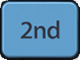
\includegraphics[width=\buttonbreite{}]{img/tiprobuttonimages/2nd.png}}}
\newcommand{\tiprobutton}[1]{\raisebox{-2mm}{\mbox{\,\includegraphics[width=\tiprobuttonbreite{}]{img/tiprobuttonimages/#1.png}\,}}}

\newcommand{\nspirebutton}[1]{\raisebox{-2mm}{\mbox{\,\includegraphics[width=\nspirebuttonbreite{}]{img/nspirebuttonimages/#1.png}\,}}}

%% Counter  für Aufgaben
%% Bei jedem Part wird die Aufgabennummer zurückgesetz auf 1
\newcommand{\bbwPartID}{AA1}
\newcommand{\bbwAufgabenBlockID}{}
\newcounter{bbwAufgabenNummerCounter}[part]
\setcounter{bbwAufgabenNummerCounter}{1}
\newcommand{\bbwAufgabenNummer}{\arabic{bbwAufgabenNummerCounter}}
\newcommand{\nextBbwAufgabenNummer}{\stepcounter{bbwAufgabenNummerCounter}}
\newcommand{\aufgSubLabel}{{\color{blue}\bbwAufgabenNummer. \alph*)}}

\newenvironment{bbwAufgabenBlock}{%% Begin environment

{\color{blue}\bbwAufgabenNummer. {\small[\bbwAufgabenBlockID]}}
\begin{enumerate}[label=\aufgSubLabel]
}{%% END Part
\end{enumerate}
\nextBbwAufgabenNummer
}%% END environment bbwAufgabenBlock

%%%%%%%%%%%%%%%%%%%%%%%%%%%%
%% Weblinks und Mathe Ninja Links

\newcommand{\weblink}[2]{\href{#2}{#1}}

\newcommand{\matheNinjaLink}[2]{
\begin{tabular}{cc}
 \raisebox{-1cm}{
\includegraphics[height=2cm]{img/matheninja/turtle.png}}& \href{#2}{MatheNinja: #1}\\
 \end{tabular} 
%%\bbwCenterGraphic{2cm}{img/matheninja/turtle.png}
%%$$\Longrightarrow \Longrightarrow \href{#1}{MatheNinja} \Longleftarrow\Longleftarrow$$
}%% End Command  \matheNinjaLink

%% Philipp G Freimann Juli 2019 für die BBW
%% Phi BBW-Vorlage für Mathematische Dokumente (LaTeX)
%% 2019 - 07 - 11
%%%%%%%%%%%%%%%%%%%%%%%%%%% M a t h e   M a k r o s %%%%%%%%%%%%%%%%%%%%%%%%%%%%%5

\usetikzlibrary{arrows.meta}

%% Kleine Symbole über anderen. Z. B. "?" über einem
%% Gleichheitszeichen:
%% Use \ueberMini{=}{?} um ein kleines Fragezeichen über ein
%% Gleichheitsszeichen zu schreiben.
\newcommand{\ueberMini}[2]{ \mathrel{\stackrel{\makebox[0pt]{\mbox{\normalfont\tiny #2}}}{#1}} }

%% Gleichungssystem mit zwei Zeilen und vier Einträgen (je zwei links
%% bzw. rechts).
\def\gleichungZZ#1#2#3#4{%%
  $$\left|
  \begin{array}{rcl}
    {#1} &=& {#2}\\
    {#3} &=& {#4}
    \end{array}\right|$$}%%

\def\gleichungDD#1#2#3#4#5#6{%%
  $$\left|
  \begin{array}{rcl}
    {#1} &=& {#2}\\
    {#3} &=& {#4}\\
    {#5} &=& {#6}\\
    \end{array}\right|$$}%%

%% Entspricht-Symbol
%%\usepackage{accents}
\newcommand{\hatset}[1]{\accentset{\wedge}{#1}}
\newcommand{\entspricht}{\,\,\hatset{=}\,\,}
\newcommand*\mittelwert[1]{\bar{#1}}
\newcommand*\mediantilde[1]{\widetilde{#1}}

%%
%% Graphiken mit tikz: BBW-Mathe-akros
%%
\tikzset{bbwgrid/.style={help lines,color=cyan!18, step=0.5cm}}

%% Koordinatensystem ohne Zahlen
\newcommand{\bbwGridPartLeer}[4]{
 % grid:
 \draw[bbwgrid] (#1,#3) grid (#2,#4);

 % axes
 \draw[thick] (#1,0) -- (#2,0);
 \draw[thick] (0,#3) -- (0,#4);
 \foreach \x in {#1, ..., -1}  \draw (\x cm, 2pt) -- (\x cm, -2pt);%%  node[anchor=north]{$\x$};
 \foreach \x in {1, ..., #2}   \draw (\x cm, 2pt) -- (\x cm, -2pt);%%  node[anchor=north]{$\x$};
 \foreach \y in {#3, ..., -1}  \draw (-2pt, \y cm) -- (2pt, \y cm);%%  node[anchor=east]{$\y\,\,$};
 \foreach \y in {1, ..., #4}   \draw (-2pt, \y cm) -- (2pt, \y cm);%%  node[anchor=east]{$\y\,\,$};
 \draw[->,thick] (#2,0) -- ({#2+0.5},0) node[anchor=west]{$x$};
 \draw[->,thick] (0,#4) -- (0,{#4+0.5}) node[anchor=south]{$y$};
}

\newcommand{\bbwGridPart}[4]{
 % grid:
 \draw[bbwgrid] (#1,#3) grid (#2,#4);

 % axes
 \draw[thick] (#1,0) -- (#2,0);
 \draw[thick] (0,#3) -- (0,#4);
 \foreach \x in {#1, ..., -1}  \draw (\x cm, 2pt) -- (\x cm, -2pt)  node[anchor=north]{$\x$};
 \foreach \x in {1, ..., #2}   \draw (\x cm, 2pt) -- (\x cm, -2pt)  node[anchor=north]{$\x$};
 \foreach \y in {#3, ..., -1}  \draw (-2pt, \y cm) -- (2pt, \y cm)  node[anchor=east]{$\y\,\,$};
 \foreach \y in {1, ..., #4}   \draw (-2pt, \y cm) -- (2pt, \y cm)  node[anchor=east]{$\y\,\,$};
 \draw[->,thick] (#2,0) -- ({#2+0.5},0) node[anchor=west]{$x$};
 \draw[->,thick] (0,#4) -- (0,{#4+0.5}) node[anchor=south]{$y$};
}


%% A function within a Grid (without painting the grid)
%% #1: funciton eg 2*\x  (x has to be backquoted)
%% #2: Domain eg. -1:2.5
%% #3: colour eg red
\newcommand{\bbwFuncC}[3]{\draw[domain=#2,smooth,samples=200,variable=\x,#3] plot ({\x},{#1});
}
%% A function within a Grid (without painting the grid)
\newcommand{\bbwFunc}[2]{\bbwFuncC{#1}{#2}{blue}}

%% Declare a function-plot
%% xmin,xmax,ymin,ymax,fct,domain(x-min, x-max)
%% example: \bbwFunction{-4}{3}{-2}{5}{-\x*\x- \x + 4.5}{-3:2}
\newcommand{\bbwFunction}[6]{\begin{tikzpicture}
\bbwGridPart{#1}{#2}{#3}{#4}
 \bbwFunc{#5}{#6}
%% \draw[domain=#6,smooth,samples=200,variable=\x,blue] plot ({\x},{#5});
\end{tikzpicture}}
%% a whole graph having a coordinate-system #1-#4 and any tizpicture content #5:
\newcommand{\bbwGraph}[5]{\begin{tikzpicture}\bbwGridPart{#1}{#2}{#3}{#4}#5\end{tikzpicture}}
\newcommand{\bbwGraphLeer}[5]{\begin{tikzpicture}\bbwGridPartLeer{#1}{#2}{#3}{#4}#5\end{tikzpicture}}

%% Dots and lines:
%% Dot example: \bbwDot{-1,2}{red}{east}{A}
\newcommand{\bbwDot}[4]{\filldraw[color=#2!60, fill=#2!5, thick](#1) circle(0.05) node[anchor=#3]{$#4$};}

%% Line example: \bbwLine{-1,0}{2,3}{red}
\newcommand{\bbwLine}[3]{\draw[thick,color=#3] (#1)--(#2);}

\newcommand{\bbwArrow}[3]{\draw[thick,color=#3,->] (#1)--(#2);}


%% Draw a single letter or small text
% #1: Position eg  4,4
% #2: letter eg f or blah
% #3: colour
\newcommand{\bbwLetter}[3]{\draw[color=#3](#1) node{$#2$};}

%%% ABC-Formel
%% usage \abcd{<a>}{<b>}{<c>}
%% example usage: \abcd{b}{5}{\sqrt{4}}
\newcommand{\abcd}[3]{$\frac{-(#2)\pm\sqrt{(#2)^2 - 4\cdot{}(#1)\cdot{}(#3)}}{2\cdot{}(#1)}$}



%% Trigonometrische Koordinatensysteme
%% Alle heißen "trigsysS" wobei da S einer der folgenden Sub-Systeme
%% bezeichnet:
%%  A  phi von  0 ... 360
%%     y   von -3 ...   3
%%
%%  B  phi von  0 ... 360
%%     y   von -1 ...   1
%%
%%  C  phi von  -270 ... 450
%%     y   von    -2 ...   2
%%
%%  D  phi von  -270 ... 450
%%     y   von    -1 ...   1
%%

%% coordSysBBWFlex
%% Flexibles Koordinatensystem mit Pfeilen und Pfeilbeschriftung, aber
%% noch ohne "ticks".
%% #1   : Rastergröße
%% #2-#5: Größe des Rasters in cm
%% #6   : Beschriftung in x-Richtung (in y-Richtung ist es immer y
%% #7   : Zu zeichnende Funktion
%% #8   : Ticks oder was sonst noch komplexeres in die Grafik muss
\newcommand{\bbwFunctionColour}{blue}
\newcommand{\coordSysBBWFlex}[8]{
\begin{tikzpicture}
\draw[step = #1,  thin, cyan!20] (#2, #4) grid (#3, #5);
\draw[thick, ->] (#2,0) -- (#3,0) node[anchor = west] {$#6$};
\draw[thick, ->] (0,#4) -- (0,#5) node[anchor = south] {$y$};
\draw[domain=#2:#3,smooth,samples=200,variable=\x,\bbwFunctionColour] plot ({\x},{#7});
#8;
\end{tikzpicture}
\renewcommand{\bbwFunctionColour}{blue}
}%% end coordSysBBW

%% Koordinatensystem von 0 - 360 Grad (y -Ricthung -1 bis 1
%% Die Funktion kann mit dem 1. Parameter eingegeben werden
\newcommand{\trigsysAFct}[1]{
\coordSysBBWFlex{0.5cm}{-1}{13}{-4}{4}{\varphi}{#1}{
  \foreach \x [evaluate=\x as \degree using int(\x*30)] in {1,...,12}{ 
    \draw (\x cm, 1pt) -- (\x cm, -1pt) node[anchor = north] {$\degree^\circ$};
  }
  \foreach \y in {-3,-2,-1,1,2,3}{
   \draw (1pt, \y cm) -- (-1pt, \y cm) node[anchor = east] {$\y$};
  }
}
}%% end trigsysC

%% Leeres Koordinatensystem (fct = 0)
\newcommand{\trigsysA}{\trigsysAFct{0}}


%% Koordinatensystem von -270 bis 450 Grad. In y-Richtung von -2 bis 2
%% Funktion wird mit #1-Parameter angegeben
\newcommand{\trigsysBFct}[1]{
\coordSysBBWFlex{0.5cm}{-1}{13}{-4}{4}{\varphi}{#1}{
  \foreach \x [evaluate=\x as \degree using int(\x*30)] in {1,...,12}{ 
    \draw (\x cm, 1pt) -- (\x cm, -1pt) node[anchor = north] {$\degree^\circ$};
  }
  \foreach \y in {-1,1}{
   \draw (1pt, \y *3cm) -- (-1pt, \y *3cm) node[anchor = east] {$\y$};
  }
}
}%% end trigsysC

%% Leeres B-System
\newcommand{\trigsysB}{\trigsysBFct{0}}


%% Wie B-SYstem, jedoch in y-Richtung von -1 bis +1
\newcommand{\trigsysCFct}[1]{
\coordSysBBWFlex{0.2cm}{-6}{10}{-2.5}{2.5}{\varphi}{#1}{
  \foreach \x [evaluate=\x as \degree using int(\x*90)] in {-3,-2,-1,1,2,3,4,5}{ 
   \draw (\x *18mm, 1pt) -- (\x * 18mm, -1pt) node[anchor = north] {$\degree^\circ$};
  }
   
  \foreach \y in {-2,-1,1,2}{
    \draw (1pt, \y cm) -- (-1pt, \y cm) node[anchor = east] {$\y$};
  }
}
}%% end trigsysC

\newcommand{\trigsysC}{\trigsysCFct{0}}


\newcommand{\trigsysDFct}[1]{
\coordSysBBWFlex{0.2cm}{-6}{10}{-2.5}{2.5}{\varphi}{#1}{
 \foreach \x [evaluate=\x as \degree using int(\x*90)] in {-3,-2,-1,1,2,3,4,5}{ 
   \draw (\x *18mm, 1pt) -- (\x * 18mm, -1pt) node[anchor = north] {$\degree^\circ$};
  }   
  \foreach \y in {-1,1}
   \draw (1pt, \y *2cm) -- (-1pt, \y *2cm) node[anchor = east] {$\y$};
  }
} %% end command: trig sys D cos()


\newcommand{\trigsysDcos}{\trigsysDFct{2*cos(\x*50)}}
\newcommand{\trigsysDsin}{\trigsysDFct{2*sin(\x*50)}}
\newcommand{\trigsysD}{\trigsysDFct{0}}




%% LAYOUT FUER ARBEITSBLAETTER %%
\headheight12mm

%%%%%%%%%%%%%%%  H E A D E R   &   F O O T E R %%%%%%%%%%%%%%%%%%%%

%% Headers
\fancyhf[HL]{\makebox{
\includegraphics[width=30mm]{logos/bbw.pdf}}}
\fancyhf[HC]{\metaHeaderLine{}}
\fancyhf[FR]{\tiny{fp @ bbw}}

\newcommand{\arbeitsblattHeader}{
  \begin{center}
    {\Large \fontfamily{qhv}\selectfont \arbeitsblattTitel{}}
\end{center}}


%%%%%%%%%%%%%%%%%%%%%%%%%%%%%%%%%%%%%%%%%%%%%%%%%%%%%%%%%%%%%%%%%%

%%\usepackage{amssymb} %% für \blacktriangleright
\usepackage{makecell}
\renewcommand{\metaHeaderLine}{Formelsammlung (v 0.0.26 2021-06-20 fp)}
\renewcommand{\arbeitsblattTitel}{Formelsammlung GeSo}

\titlespacing*{\section}{0pt}{0.1\baselineskip}{0.1\baselineskip}
\titlespacing*{\subsection}{0pt}{0.1\baselineskip}{0.1\baselineskip}



%%% MODERN:
\renewcommand{\rmdefault}{phv} % Arial
\renewcommand{\sfdefault}{phv} % Arial
\definecolor{fsgray}{HTML}{eeeeee}
\renewcommand{\rezeptFarbe}{fsgray}
%%\renewcommand{\definitionFarbe}{fsgray}
\renewcommand{\gesetzFarbe}{fsgray}
\renewcommand{\beispielFarbe}{fsgray}
\renewcommand{\bemerkungFarbe}{fsgray}
%%% END MODERN


%% Benutze
%%\columnbreak
%% für harten Break:
%% Force column-break
\newcommand{\forceCB}{\vfill\null\columnbreak}

\begin{document}%%
\arbeitsblattHeader{}

\begin{multicols}{2}%%

\section*{Zahlmengen}
\begin{definition*}{}{}
Die Zahlmengen heißen

$\mathbb{N} = \{1,2, ...\}$                                   \textbf{natürlich}\\
$\mathbb{Z} = \{..., -2, -1, 0, 1,2, ...\}$                   \textbf{ganz}\\
$\mathbb{Q} = \{\frac{a}b|a\in \mathbb{Z},b\in\mathbb{N}\}$   \textbf{rational} (Brüche)\\
$\mathbb{R} = \{..., -1, ..., 0, ... \frac12, ..., \sqrt{2}, ..., e, ... \pi, ...\}  $ \textbf{reell} (alle Zahlen auf der Zahlengerade)\\

\textbf{Prim}zahl: hat genau zwei Teiler (Eins und sich selbst):\\ $\mathbb{P} = \{2, 3, 5, 7, 11, 13, ...\}$
\end{definition*}

$$\mathbb{P} \subset \mathbb{N} \subset \mathbb{Z} \subset \mathbb{Q} \subset \mathbb{R}$$

\TRAINER{$|\mathbb{N}| = |\mathbb{Q}|$ aber $|\mathbb{Q}| \ne |\mathbb{R}|$} 

\hrulefill%% hrulefill vor allen neuen "sections" auf derselben Seite

\section*{Algebra}

\subsection*{Grundrechenarten}
$$3-(-7) = +10$$
aber
$$-3(-7) = +21$$

\begin{gesetz*}{Binomische Formeln}{}
$$(a+b)^2 = a^2+2ab + b^2$$%%
$$(a-b)^2=a^2-2ab+b^2$$%%
$$(a-b)\cdot(a+b) = a^2 - b^2$$
Bsp.:
$$1-x^2 = (1-x)\cdot{}(1+x)$$
\end{gesetz*}

\subsection*{Vertauschte Differenz}
($-1$ ausklammern)

$(b-a)=(-1)\cdot{}(a-b)$

Beispiel:

$\frac{x}{a-b} +  \frac{y}{b-a} = \frac{x}{a-b} + \frac{-y}{a-b} = \frac{x-y}{a-b}$

%% Forced column break
%%\forceCB
\subsection*{Summenzeichen}
%%$$\color{orange}\sum_{\color{blue}k=1}^{\color{blue}n} {{\color{ForestGreen}T}(k)} = {\color{ForestGreen}T}({\color{blue}1}) {\color{orange}+} {\color{ForestGreen}T}({\color{blue}2}) {\color{orange}+} ... {\color{orange}+} {\color{ForestGreen}T}({\color{blue}n})$$

  $${\color{green}\sum_{{\color{red}k}{{\color{green}{\color{black}=}\color{blue}1}}}^{\color{blue}n\color{green}}}
  {\color{orange}T(}{{\color{red}k}}{\color{orange})} = {\color{orange}T(}{\color{blue}1}{\color{orange})} {\color{green}+} {\color{orange}T(}{\color{blue}2}{\color{orange})} {\color{green}+}
  ... {\color{green}+} {\color{orange}T(}{\color{blue}n}{\color{orange})}$$

Beispiel

  $${\color{green}\sum_{{\color{red}n}{{\color{green}{\color{black}=}\color{blue}3}}}^{\color{blue}5\color{green}}}  {\color{red}n}^{{\color{orange}7}} = {\color{blue}3}^{\color{orange}7} {\color{green}+} {\color{blue}4}^{\color{orange}7} {\color{green}+} {\color{blue}5}^{\color{orange}7}$$


Taschenrechner: \tiprobutton{math} 4 \texttt{ sum}


\subsection*{(Absolut)betrag einer Zahl}

$|7| = 7$;  \hfill{ } $|-5| = 5$; \hfill{} $-|6|=-6$; \hfill{} $-|-4| = -4$

\TRAINER{Intervall-Schreibweise? \zB $a\in[0;1[$}

\hrulefill

\section*{Dezimalzahlen}
\subsection*{Runden}
Runden auf \textbf{\color{ForestGreen}vier}  Dezimalen: betrachte die nächste Ziffer und runde auf, falls diese {\color{red}Ziffer} $\ge 5$.

Beispiel

$3.\textbf{\color{ForestGreen}4729}\textbf{\color{red}6}44 \approx
3.\textbf{\color{ForestGreen}4730}$; \hfill{ }
$70.\textbf{\color{ForestGreen}0031}\textbf{\color{red}4}998\approx
70.\textbf{\color{ForestGreen}0031}$

(Alle vier Dezimalen sind anzugeben.)

\subsection*{Signifikante Stellen}
Führende Nullen zählen nicht, nachfolgende Nullen
zählen. Bsp. \textbf{\color{ForestGreen}drei} signifikante Stellen:

\textbf{\color{ForestGreen}208} cm = \textbf{\color{ForestGreen}2.08} m = 0.00\textbf{\color{ForestGreen}208} km

Bsp.: Runden auf \textbf{\color{ForestGreen}vier} signifikante Stellen:

\textbf{\color{ForestGreen}208.6}\textbf{\color{red}6} cm $\approx$ \textbf{\color{ForestGreen}208.7} cm

0.00\textbf{\color{ForestGreen}2086}\textbf{\color{red}6} km $\approx$ 0.00\textbf{\color{ForestGreen}2087} km


\textbf{\color{ForestGreen}30.89}\textbf{\color{red}6} $\approx$ \textbf{\color{ForestGreen}30.90}

(4. Ziffer stehen lassen, auch wenn = 0)

%%\forceCB{}%%
\subsection*{Wissenschaftliche Notation}
Für große, aber auch für Zahlen sehr nahe an 0, wird die wissenschaftliche Schreibweise vorgezogen. Dabei steht vor dem Dezimalpunkt immer \textbf{\color{blue}genau eine Ziffer}:

\begin{tabular}{lcccr}
Zahl  & & wissenschaftl. & & TR: \tiprobutton{EE} \\
3400  &=& $\textbf{\color{blue}3}.4\cdot{}10^3$ &=& {\textbf{\color{blue}3}}.4E3\\
0.004 &=& $\textbf{\color{blue}4}\cdot{}10^{-3}$ &=&\textbf{\color{blue}4}E-3\\
\end{tabular}

\section*{Bruchterme}
\subsection*{Faktorisieren}


\begin{rezept*}{}{}
\begin{enumerate}
\item gemeinsame Faktoren ausklammern
$$\frac{ax+ay}{bx+by} =\frac{a(x+y)}{b(x+y)} = \frac{a}b$$
\item Teilsummen ausklammern
$$3(7r+6) - b(7r+6) = (3-b)(7r+6)$$
\item Binomische Formeln
$$x^2-1 = (x-1)(x+1)$$
$$4b^2-9c^2=(2b+3c)(2b-3c)$$
\item Zweiklammeransatz
$$x^2+2x-15 = (x+5)(x-3)$$
Die Faktoren für den Zweiklammeransatz können mit dem Taschenrechner
gefunden werden:\\ a) \texttt{poly-solv} \tiprobutton{cos_poly-solv}
oder\\ b) \texttt{PFactor} \tiprobutton{math}\tiprobutton{4}

\textbf{\color{red}Achte auf Vorzeichen!}
\end{enumerate}
\end{rezept*}


\section*{Potenzen}
\begin{definition*}{Potenz}{}
$$a^n := \underbrace{a\cdot{}a\cdot{}a\cdot{}...\cdot{}a}_{n\textrm{ Faktoren}}$$
$$7^3=7\cdot{}7\cdot{}7=343$$
$7^3$ Potenz\\
$7$ Basis\\
$3$ Exponent\\
$343$ Potenzwert\\
\end{definition*}

\begin{gesetz*}{gleiche\,Basis}{}
\begin{tabular}{cc}
$a^m\cdot{}a^n = a^{m+n},$ & $a^m:a^n=a^{m-n},$ \\
$\left(a^m\right)^n = a^{m\cdot{}n}$ &\\
 \end{tabular} 
\end{gesetz*}

\begin{gesetz*}{gleicher\,Exponent}{}
\begin{tabular}{cc}
$a^n\cdot{}b^n = (a\cdot{}b)^n,$ & $\frac{a^n}{b^n} =\left(\frac{a}b\right)^n $\\
 \end{tabular}
\end{gesetz*}

\subsection*{Vorzeichen}
Fall: $n$ \textbf{gerade}:

\begin{tabular}{cc}
 $-(a^n) = -a^n,$ & aber: $(-a)^n = +a^n$\\
 \end{tabular} 

Fall: $n$ \textbf{un}gerade:

\begin{tabular}{cc}
 $-(a^n) = -a^n,$ & aber: $(-a)^n = -a^n$\\
 \end{tabular} 


\begin{gesetz*}{negative Exponenten}{}

Für Basis $a\ne 0, b\ne 0$ und $m \in\mathbb{Q}$ gilt:

\begin{tabular}{ccc}
$a^0=1,$ & $a^{-m} = \frac1{a^m},$ & $\left(\frac{a}b\right)^{-m} = \left(\frac{b}a\right)^m$ \\
 \end{tabular}
\end{gesetz*}

\begin{rezept*}{}{}{}
Exponenten vertauschen ihr Vorzeichen beim Übertreten des Bruchstrichs:
$$\frac{a^{-3}b^2}{c^5d^{-6}} = \frac{b^2d^6}{a^3c^5}$$
\end{rezept*}

\subsection*{$n$-te Wurzel}
$\sqrt[n]{a} := \left(a\right)^\frac1n$\hfill{}Bsp.: $8^{\frac13}=\sqrt[3]{8}=2$
\begin{gesetz*}{}{}
$$a^{\frac{m}n} = \sqrt[n]{a^m} = \left(\sqrt[n]a\right)^m$$
\end{gesetz*}%%
%%

%%\forceCB%%
\hrulefill
\section*{Logarithmen}

\begin{definition*}{$\log$}{}

Für $a>0, a\ne 1$ ist

$$\log_a{}(z)=x \Longleftrightarrow{} a^x = z$$
\end{definition*}
$a$ = Basis, $z$ = Numerus (stets > 0), $x$ = Logarithmus (= Exponent in der Potenzschreibweise)

Logarithmen sind Exponenten zu einer fest gewählten Basis.

\begin{gesetz*}{}{}
$$\log_a(u\cdot v) = \log_a(u) + \log_a(v)$$
$$\log_a(u : v) = \log_a(u) - \log_a(v)$$
$$\log_a(b^x) = x\cdot{}\log_a(b)$$
\end{gesetz*}

\subsection*{Spezielle Werte}
\begin{tabular}{ccc}
$\log(1)=0$     &    $\lg(10) = 1$ & $\lg(1000)=3$           \\
$\lg(0.01)=-2$ & $\log_a(a) = 1$   & $\ln(e) = 1$\\
\end{tabular}
\begin{gesetz*}{Basiswechsel}{}
$$\log_{\color{ForestGreen}a}({\color{red}b}) = \frac{\lg({\color{red}b})}{\lg({\color{ForestGreen}a})} = \frac{\ln({\color{red}b})}{\ln({\color{ForestGreen}a})}$$
\end{gesetz*}
\hrulefill
\section*{Gleichungen}

\subsection*{Lineare Gleichungen}
\TRAINER{Ist das Beispiel nötig? Sollen sie selbst?}
\TRAINER{Wollen wir so viele Beispiele???}
$$5x-3a = 2cx-7b$$
1. Alle $x$ nach links, übriges rechts:
$$5x - 2cx = 3a-7b$$
2. $x$ \textbf{\color{red}ausklammern}
$$x\cdot{}{\color{red}(5-2c)} = 3a-7b$$
3. Durch Klammer teilen
$$x = \frac{3a-7b}{{\color{red}5-2c}}$$


\subsection*{num-solv}
Der Taschenrechner löst Gleichungen mit Zahlen nach $x$ auf:

$5^x = 100 -x$; verwende \tiprobutton{2nd}\tiprobutton{sin_num-solv} $x\approx{}2.843$



\subsection*{Bruchgleichungen}

\begin{definition*}{}{}

\textbf{Definitionsbereich} $\mathbb{D}$: welche Werte dürfen in einen Term eingesetzt werden

Bsp. Nenner darf nicht Null werden:

Bsp.: $$\frac5{x+2}=\frac{7+x}{x-3} \Leftrightarrow{} \mathbb{D}_x=\mathbb{R}\backslash{}\{-2, 3\}$$
\end{definition*}

\begin{rezept*}{}{}
\begin{enumerate}
\item Definitionsbereich $\mathbb{D}$ finden
\item Faktorisieren und kürzen, dann...
\item ... Hauptnenner finden,
\item lösen und 
\item Schlusskontrolle!
\end{enumerate}
\end{rezept*}


\forceCB
\subsection*{Quadratische Gleichungen}
\begin{gesetz*}{Lösungsformel}{}
\textbf{Grundform}: $ax^2 + bx+c = 0$

$$x_{1,2} = \frac{-b \pm \sqrt{b^2-4ac}}{2a}$$
\end{gesetz*}

\textbf{Diskriminante} $D = b^2-4ac$:
$D>0$: Zwei Lösungen;
$D=0$: Eine Lösung;
$D<0$: Keine Lösung


Taschenrechner \tiprobutton{2nd}\tiprobutton{cos_poly-solv}\\

\hrulefill

\subsection*{Potenzgleichungen}

$$x^a=c \Leftrightarrow x=\sqrt[a]{c}$$

Allgemein

$$x^{\frac{a}b} = c \Leftrightarrow{}
x=c^{\frac{b}a} = \sqrt[a]{c^b}$$

\subsection*{Exponentialgleichungen}
\textbf{Fall 1} Exponentenvergleich. Bsp.:

$$5^4=125^x \Rightarrow{} 5^4=(5^3)^x \Rightarrow{} 5^4=5^{3x} \Rightarrow{}$$
$$ 4=3x \Rightarrow x=\frac43$$

\textbf{Fall 2} Logarithmen. Bsp.:

$$5\cdot{}7^x=105 \Leftrightarrow 7^x=21 \Rightarrow x=\log_7(21)$$
oder so (mit Zehnerlogarithmus $(\lg)$):
$$5\cdot{}7^x=105 \Rightarrow$$
$$7^x=21 \Rightarrow$$
$$ \lg(7^x)=\lg(21) \Rightarrow$$
$$x\cdot{}\lg(7)=\lg(21) \Rightarrow$$
$$ x=\frac{\lg(21)}{\lg(7)}$$

\begin{rezept}{Taschenrechner}{}
$\lg$ auf Taschenrechner: «\texttt{log(}» mit der \tiprobutton{ln_log}-Taste (2$\times$ drücken)
\end{rezept}

\begin{gesetz*}{Exponentialgleichung}{}
$$a^x=b \Rightarrow{} x=\log_a(b) = \frac{\lg(b)}{\lg(a)}$$
\end{gesetz*}


\subsection*{Lineare Gleichungssysteme}
Erst in \textbf{Grundform} bringen und dann
\gleichungZZ{5x+7y}{19}{16x -13y}{-4}
mit Taschenrechner «\texttt{sys-solv}» \tiprobutton{2nd}\tiprobutton{tan_sys-solv} lösen.

Verfahren
\begin{itemize}
\item Einsetzungsverfahren
\item Additionsverfahren
\item Gleichsetzungsverfahren
\item Graphische Lösung mit zwei Geradengleichungen
\item Substitution:
\end{itemize}

\subsection*{Substitution}
Beispiel Bruchgleichungssysteme:

\gleichungZZ{{\color{ForestGreen}\frac1{x+1}} + {\color{orange}\frac3{y-2}}}{66}{{\color{ForestGreen}\frac2{x+1}} + {\color{orange}\frac5{y-2}}}{16}
Substituiere
${\color{ForestGreen}a}:={\color{ForestGreen}\frac1{x+1}}$ und
${\color{orange}b} : ={\color{orange}\frac1{y-2}}$:
\gleichungZZ{{\color{ForestGreen}a} + 3{\color{orange}b}}{66}{2{\color{ForestGreen}a} + 5{\color{orange}b}}{16}

Dann: Rücksubstitution


\hrulefill
\section*{Textaufgaben}
\subsection*{Geschwindigkeitsaufgaben}
\fbox{$s = v\cdot{} t$} (Einheiten kompatibel wählen!)

\subsection*{Leistungsaufgaben}
Bei $x$ Zeiteinheiten für die ganze Arbeit:

Leistung = Arbeit pro Zeiteinheit

Leistung = $\frac{1 \textrm{ [Arbeit]}}{x \textrm{ [Zeiteinheiten]}}$

Physik: Leistung = $\frac{\textrm{[Joule]}}{\textrm{[Sekunde]}} = [\textrm{Watt}]$

\subsection*{Restaufgaben}
$$A:B = C \textrm{ Rest } R \Longleftrightarrow{}  C\cdot{}B+R = A$$
\TRAINER{Restaufgaben: Noch stehen gelassen, da im Kompendium oder in alter Prüfung gesichtet.}


\subsection*{Zinseszins}
\begin{itemize}
\item $K_0$ = Startkapital; $K_n$ = Endkapital
\item $p$ = Zinssatz (in \%);\\ $a = 1+\frac{p}{100}$ = Zinsfaktor
(Wachstumsfaktor);\\ $p<0$, so ist $a$ der Zerfallsfaktor
\end{itemize}
$$K_n = K_0 \cdot{} \left( 1+\frac{p}{100} \right)^n = K_0\cdot{}a^n$$

\subsubsection*{Beispiele}
$$p = 2.5\% \Longleftrightarrow{} a = 1.025$$
$$p = -3\% \Longleftrightarrow{}  a = 0.97 $$

\hrulefill
\section*{Funktionen}
\TRAINER{Brauchen wir diese Definition???}

Eine Funktion ordnet jeder Zahl aus einem Definitionsbereich
$\mathbb{D}$ \textbf{genau} eine Zahl aus einem Wertevorrat
$\mathbb{W}$ (=Zielmenge) (meist $\mathbb{R}$) zu.

\hrulefill
\section*{Lineare Funktionen}
Explizite Form:
$$g: y = f(x) = a\cdot{}x + b$$

\bbwCenterGraphic{8cm}{img/lineareFunktion.png}
$a$ = Steigung = $\frac{V}{H}=\frac{\Delta y}{\Delta x} = \frac{y_2-y_1}{x_2-x_1}$.\\
Zwei Geraden sind \textbf{parallel}, wenn ihre Steigungen gleich sind.

$b$ = $y$-Achsenabschnitt (=Ordinatenabschnitt)


\subsection*{Nullstelle...} ...einer Funktion: $y=0$ setzen und nach $x$
auf\/lösen.

Bsp.: $y=7x+4$ Nullstelle: $0 = 7x+4$, d.\,h. $x_0=\frac{-4}{7}$

\subsection*{Ordinatenabschnitt}
\textbf{Schnittpunkt mit der $y$-Achse}: $x=0$ setzen.

Bsp.: $y=7x+4$ Achsenabschnitt = Schnittpunkt mit der $y$-Achse:
$x=0$.\\
Also $y=7\cdot{}0 + 4 = 4$. Somit liegt der Schnittpunkt bei $(0|4)$.


\subsection*{Schnittpunkt zweier Geraden}
Gegeben: $g: y=ax+b$ und $h: y=cx+d$.

Gleichsetzen: $ax+b = cx+d$


\subsection*{Mittelpunkt $M$ einer Strecke $AB$}
Gegeben $A=(x_A|y_A)$ und $B=(x_B|y_B)$

Gesucht Mittelpunkt $M=(x_M|y_M)$

Lösung Mittelwert $x$ und $y$ separat:

$$x_M = \frac{x_A+x_B}2; y_M=\frac{y_A+y_B}2$$

\subsection*{Horizontale Gerade}

$g: y=ax+b$ ist horizontal, wenn die Steigung $a$ wegfällt ($a=0$).

$$g:  y=0\cdot{}x+b \Rightarrow y=b$$

\subsection*{Zweipunkte Aufgaben}
Gesucht Gerade $g: y=ax+b$ durch zwei gegebene Punkte $A=(x_A|y_A)$
und $B=(x_B|y_B)$

\textbf{Variante 1}: Steigung $a = \frac{V}H = \frac{\Delta y}{\Delta x}
= \frac{y_B-y_A}{x_B-x_A}$ berechnen und einen der beiden Punkte in
$y=ax+b$ einsetzen, um $b$ zu finden.

\textbf{Variante 2}: Gleichungssystem nach $a$ und $b$ auf\/lösen:
\gleichungZZ{y_A}{a\cdot{}x_A+b}{y_B}{a\cdot{}x_B + b}

\hrulefill

\section*{Potenzfunktionen}

\begin{definition*}{Potenzfunktion}{}
Grundform:
$$y=ax^z$$
$z\in\mathbb{Z}\backslash\{0,1\} = \{...-2, -1, 2, 3, 4, ...\}$
\end{definition*}

$z>0$: Parabeln

\bbwCenterGraphic{8cm}{PotenzFktx2x4.pdf}
\TRAINER{Klarer beschriften, welche Funktion zu was und keine
Überlappungen: Insb. die Zeichen 3 und = liegen jetzt übereinander.}


$z<0$: Hyperbeln

\bbwCenterGraphic{8cm}{PotenzFkt1overx3x5.pdf}


\TRAINER{Braucht es hier noch mehr Geraden \textbf{mit}
Kooridinatensystem? Reichen nicht die folgenden qualitativen Graphiken?}

$z$ gerade: Gespiegelt an der $y$-Achse

$z$ ungerade: Gespiegelt am Ursprung $O=(0|0)$

Ist ${\color{green}a>0}$ (links in der Graphik) so sind Graphen mit
geraden Exponenten nach oben geöffnet bzw. mit ungeraden Exponenten im
Quadranten I und III.

Ist ${\color{red}a<0}$ (rechts in der Graphik) so sind Graphen mit
geraden Exponenten nach unten geöffnet bzw. mit ungeraden Exponenten
im Quadranten II und IV.

 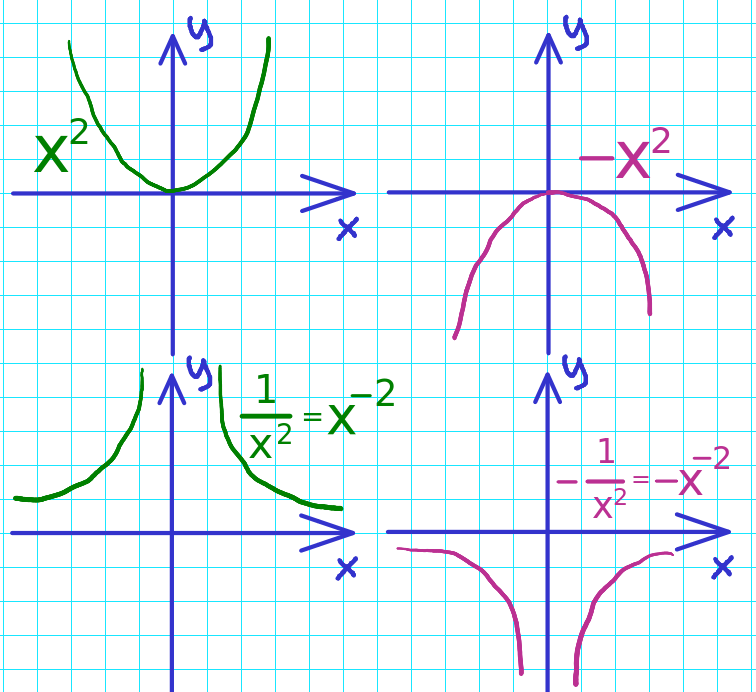
\includegraphics[width=4cm]{allg/funktionen/img/potenzfct/potenzFunktionenGerade.png}\hfill{}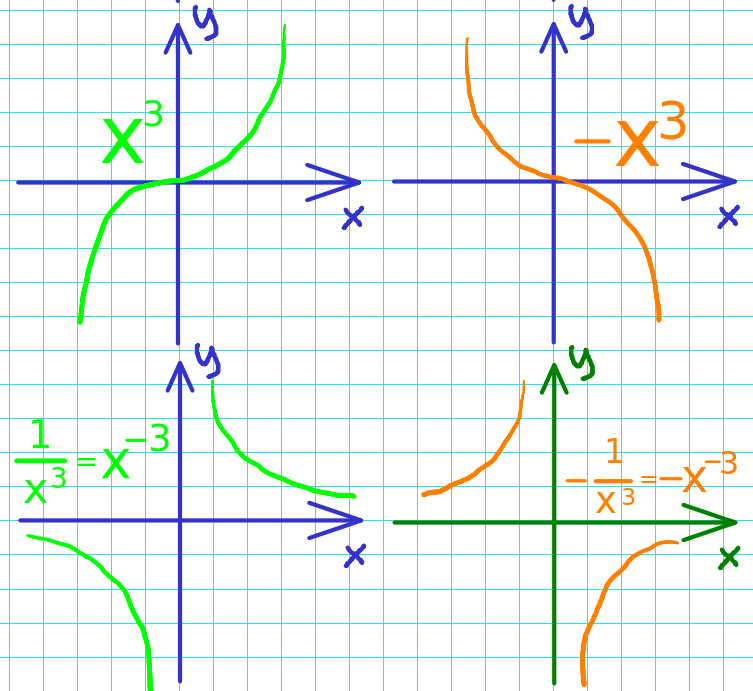
\includegraphics[width=4cm]{allg/funktionen/img/potenzfct/potenzFunktionenUngerade.png}


\hrulefill  
\subsection*{Quadratische Funktion}
$$y=ax^2$$
$a$ heißt Öffnung ($a<0$: Die Parabel ist nach unten geöffnet)

$a=1$ oder $a=-1$: Normalparabel

\hrulefill
\section*{Exponentialfunktionen}
\begin{definition*}{Exponentialfunktion}{}
$$f(t) = b\cdot{}a^t$$
$b$ = Anfangswert bei $t_0=0$; $b=f(0)$\\
\phantom{$b$} = $y$-Achsenabschnitt\\
$a$ = Vervielfältigungsfaktor ($a\in\mathbb{R}^{+}$)\\\
$a>1$: Wachstumsrate\\
$0<a<1$: Zerfallsrate
\end{definition*}

Wachstum:
\bbwCenterGraphic{8.5cm}{allg/funktionen/img/exp/exponentielles_wachstum.png}
Zerfall:
\bbwCenterGraphic{7.5cm}{allg/funktionen/img/exp/exponentieller_zerfall.png}
\begin{rezept*}{Beobachtungsintervall}{}
$$f(t) = {\color{blue}b}\cdot{}{\color{red}a}^{\frac{t}{\color{ForestGreen}\tau}}$$
$\color{ForestGreen}\tau$ = Beobachtungsintervall zu $\color{red}a$\\
$\color{red}a$ = Wachstums(/Zerfalls)rate im Zeitraum $\color{ForestGreen}\tau$

Beispiel: Die Algen mit Startwert von ${\color{blue}3} \textrm{ m}^2$ ver{\color{red}vier}fachen
sich alle {\color{ForestGreen}fünf} Tage:\\
${\color{blue}b}={\color{blue}3}$, ${\color{red}a}={\color{red}4}$, ${\color{ForestGreen}\tau}={\color{ForestGreen}5}$
$$f(t)= {\color{blue}3}\cdot{}{\color{red}4}^\frac{t}{\color{ForestGreen}5}$$
\end{rezept*}


\begin{gesetz*}{Basis $e$ Zeitvariable oft $x$}{}

$$c+b\cdot{}a^x = c + b\cdot{}e^{mx} \textrm{ mit } m = \ln(a)$$

bzw.

$$c+b\cdot{}a^\frac{x}\tau = c+b\cdot{}e^{mx} \textrm{ mit }
m=\ln(a^\frac1\tau) = \frac1\tau \cdot{}\ln(a)$$

\end{gesetz*}

\subsection*{Halbwertszeit}
$\frac12 \cdot{} b = f(t) = b\cdot{}a^{\frac{t}{\tau}}$
$$t_{\frac12} = \tau\cdot{}\log_a\left(\frac12\right)$$

\subsection*{Verdopplungszeit}
$2\cdot{}b = f(t) = b\cdot{}a^{\frac{t}{\tau}}$
$$t_{2} = \tau\cdot{}\log_a(2)$$

\subsection*{Sättigungsfunktionen}
\begin{gesetz*}{Beschränkter Zerfall}{}
$$f(t) = c + b\cdot{}a^\frac{t}\tau$$
$c$: Sättigungsgrenze\\
$0<a<1$: Zerfallsrate\\
$b$: Sättigungsdefizit bei $t=0$\\
$c+b$ = Startwert 
\end{gesetz*}


\bbwCenterGraphic{7.5cm}{allg/funktionen/img/saettigung/saettigungskurveDown.png}

\begin{gesetz*}{Beschränktes Wachstum}{}
$$f(t) = c - b\cdot{}a^\frac{t}\tau$$
$c$: Sättigungsgrenze\\
$0<a<1$: Zerfallsrate\\
$b$: Sättigungsdefizit bei $t=0$\\
$c-b$: Startwert
\end{gesetz*}

\bbwCenterGraphic{7.5cm}{allg/funktionen/img/saettigung/saettigungskurve.png}

\begin{bemerkung*}{Sättigungsdefizit}{}

$b$ = Sättigungsdefizit bei $t=0$.\\
$b\cdot{}a^\frac{t}\tau = m_t$ = Sättigungsdefizit zur Zeit $t$
\end{bemerkung*}

\end{multicols}

\hrulefill
\section*{Datenanalyse}

\subsection*{Skalen}
\bbwCenterGraphic{17cm}{img/Skalentyp.pdf}
%%\bbwCenterGraphic{15cm}{img/DatenanalyseSkalentypen.eps}
\TRAINER{Stetig/Diskret?}
\TRAINER{Mögliche Diagramm-Arten?}
\vspace{5mm}


\hrulefill
\begin{multicols}{2}

\subsection*{Lagemaße}
\subsubsection*{Mittelwert}
(= Durchschnitt = arithmetisches Mittel)

\begin{definition*}{Mittelwert}{}
$$\overline{x} = \frac{x_1 + x_2 + x_3 + ... + x_n}{n}= \frac{\sum_{k=1}^nx_n}n$$
\end{definition*}

\subsubsection*{Median}
\begin{definition*}{Median}{}
Der \textbf{Median} (Zentralwert) ist der Wert in der Mitte der geordneten Datenreihe. Ist
die Anzahl Werte gerade, so wird der Mittelwert der beiden in der
«mittleren» Werte genommen.

Symbol: $\mediantilde{x} = x_{\textrm{MED}}$
\end{definition*}

\subsubsection*{Quartil}

\begin{rezept*}{Quartile}{}

Die Quartilsgrenzen $Q_1$ bzw. $Q_3$ sind die Mediane der linken,
bzw. rechten Datenhälfte (nachdem der eine Zentralwert entfernt
wurde).

Am einfachsten mit dem Taschenrechner:

Dateneingabe: \tiprobutton{data}

Auswertung: \tiprobutton{data_stat-reg-distr}
\end{rezept*}

\subsubsection*{Modus}
Der am häufigsten auftretende Wert wird als Modus bezeichnet.

Manchmal ist dies nicht eindeutig, dann sprechen wir von einer
\textbf{multimodalen} Verteilung. Bei zwei Modi von \textbf{bimodal}.

\subsubsection*{Maximum, Minimum}
Maximum bzw. Minimum sind höchste bzw. kleinste Datenwerte: Die Ausreißer
zählen hier mit!

\subsection*{Streumaße}
\subsubsection*{Spannweite}
Die Spannweite $R$ (Range) ist das Maximum minus
das Minimum.

\subsubsection*{Interquartilsabstand}
Der Abstand zwischen $Q_1$ und $Q_3$ wird als
Quartilsdifferenz \textbf{QD} oder
englisch \textit{Interquartil-range} = \textbf{IQR} bezeichnet.

\subsubsection*{Standardabweichung}
Mit $\sigma$ bzw. $s$ wird die Standardabweichung bezeichnet. Sie
zeigt die Wendepunkte der Normalverteilung an.

$\sigma$ = Standardabweichung der Grundgesamtheit

$s$ = Standardabweichung einer gemessenen Stichprobe \TRAINER{Taschenrechner großes S}

Die Standardabweichung wird auch mit dem Taschenrechner
unter \tiprobutton{data_stat-reg-distr} gefunden.

\subsubsection*{Robustheit}
Verändert sich der Wert eines statistischen Maßes nicht, wenn sich ein Ausreißer
weiter ins Extreme bewegt, so sprechen wir von einem \textbf{robusten} Maß.
\begin{tabular}{|c|c|c|}\hline
   & Lage- & Streumaß\\\hline
 \multirow{4}{*}{\rotatebox{90}{robust}}  & Median $\mediantilde{x}$ & IQR \\
    & Modus $x_{mod}$ & \\
    & Quartile ($Q_1$,$Q_3$) & \\
    & (Ausreißerschwellen) & \\\hline
 \multirow{3}{*}{\rotatebox{90}{«fragil»}}  & Mittelwert
 $\overline{x}$ & Standardabw.: $\sigma$\\
    & Minimum & Spannweite\\
    & Maximum & \\\hline
 \end{tabular}

\subsection*{Diagramme}
\subsubsection*{Balken / Kuchen}
\begin{definition*}{Relative Häufigkeit}{}

$n$ = Anzahl Werte

$h_i$ = Absolute Häufigkeit des Merkmals $i$

$f_i = \frac{h_i}n$ = relative Häufigkeit

$p_i = f_i\cdot{}100\%$ = prozentuale Häufigkeit

$\varphi_i = f_i\cdot{}360\degre$ = Zentriwinkel im Kuchendiagramm
\end{definition*}



\subsubsection*{Histogramm}
\bbwCenterGraphic{8cm}{img/Histogramm.pdf}
\TRAINER{Ersetze «Sportler*innen» durch «Clubmitglieder»}

\begin{itemize}
\item Alle Balken sind gleich breit
\item Alle Balken berühren sich
\item Die Höhe der Balken wird durch die Häufigkeit der entsprechenden
Werte festgelegt
\item Werte auf Balkengrenzen werden immer rechts mitgezählt
\end{itemize}


\subsubsection*{Boxplot}
Vorgehen
\begin{enumerate}
\item Daten in TR eingeben \tiprobutton{data}...
\item ... und mit \tiprobutton{2nd} \tiprobutton{data_stat-reg-distr} auslesen.
\item {\color{orange} Median ($\mediantilde{x} = x_{\textrm{MED}}$)},
und Quartile ({\color{blue}$Q_1$}, {\color{green}$Q_3$})einzeichnen
\item IQR := {\color{green}Q3}-{\color{blue}Q1} rechnen
\item IQR mit 1.5 multiplizieren
\item {\color{red} untere Ausreißerschwelle\\ uAs} $ = Q_1 -
1.5\cdot{}\textrm{IQR}$\\ und {\color{red} obere Ausreißerschwelle\\ oAs} $=Q_3 + 1.5\cdot{}\textrm{IQR}$\\ (ausradierbar) fein markieren (gehören nicht zum Boxplot)
\item Alle Ausreißer mit Ring $\circ$ oder Stern $\star$ einzeichnen.
\item Whisker (entfernteste Werte innerhalb der Ausreißerschwellen)
einzeichnen.
\item Boxdekoration horizontale Linien einzeichnen.
\end{enumerate}
\bbwCenterGraphic{8cm}{img/Boxplot.pdf}

\end{multicols}
\bbwCenterGraphic{18cm}{BoxplotMitStreudiagramm.pdf}
\TRAINER{Ersetze «Sportler*innen» durch «Clubmitglieder»}
\begin{multicols}{2}
\section*{Stochastik}

\subsection*{Kombinatorik}

\subsubsection*{Produktregel}
Hat eine zweistufige Situation zunächst $k_1$ Möglichkeiten, gefolgt
von $k_2$ Möglichkeiten, so hat man insgesamt $k_1\cdot{}k_2$
Möglichkeiten. Dies ist auf beliebig viele Stufen verallgemeinerbar.

\bbwCenterGraphic{8cm}{img/KombinatorikMultiplikation.pdf}
\TRAINER{Ersetze «Ein:e Schüler:in» durch «Andrea»}

\subsubsection*{Permutationen (Sitzordnungen)}

Bei $n$ Elementen gibt es $n!$ Permutationen (=Vertauschungen):

\begin{definition*}{}{}
$$n! = n\cdot{}(n-1)\cdot{}(n-2)\cdot{}(n-3)\cdot{} ... \cdot{}2\cdot{}1$$
\end{definition*}

Bei Null Elementen gibt es nur eine Variation: $0! = 1$


\end{multicols}




\subsection*{Überblick Auswahlprobleme}
\bbwCenterGraphic{17cm}{img/Kombinatorik.pdf}

\hrulefill



\begin{multicols}{2}


\subsection*{Wahrscheinlichkeit}
\subsubsection*{Grundbegriffe}

\textbf{Ergebnismenge} $\Omega$: Menge der möglichen Ergebnisse
(Ausgänge) eines Zufallsversuchs.\\
Beispiel: Die sechs Würfelergebnise
eines Spielwürfels: $\Omega = \{\epsdice{1}, \epsdice{2}, \epsdice{3}, \epsdice{4}, \epsdice{5}, \epsdice{6}\}$

\textbf{Ereignis} $A$: Eine Teilmenge von $\Omega$. Beispiel: Eine
ungerade Zahl zu werfen: $A  = \{\epsdice{1}, \epsdice{3}, \epsdice{5}\}$

\textbf{Gegenereignis} $\overline{A} = \Omega \backslash A$ =
\textit{Gegenmenge}

$\overline{A}$ sprich «nicht» $A$.

Es gilt $A \cup \overline{A} = \Omega$

\textbf{Elementarereignis}: Ereignis bestehend aus einem einzigen
Ergebnis aus $\Omega$. Beispiel: $E_1$ = Wirf eine \textbf{Eins}: $E_1
= \{\epsdice{1}\}$.


\subsection*{Elementare Wahrscheinlichkeit}
Die Wahrscheinlichkeit des \textbf{Gegenereignisses} von $E$ ist
$$P(\overline{E}) = 1- P(E)$$
Bei Aufgaben wie «... mindestens eins ...» ist das Arbeiten mit der
Gegenwahrscheinlichkeit häufig einfacher.

Ereignisse sind voneinander \textbf{unabhängig}, wenn sie keine
gleichen Ergebnisse aufweisen.
$$A \textrm{ unabhängig von } B \Leftrightarrow A\cap B=\{\}$$

Für voneinander \textbf{unabhängige} Ergebnisse 
gilt:

$$P(A\textrm{ «oder» }B) = P(A\cup B) = P(A) + P(B)$$


\subsubsection*{Baumdiagramme}

\textbf{Pfadregel}:
Entlang eines Pfades (Äste hintereinander) multiplizieren sich die
Wahrscheinlichkeiten.

\textbf{Summenregeln}:
\begin{itemize}
\item Alle von einem Knoten ausgehenden Wahrscheinlichkeiten haben in
der Summe 100\%, also $P=1.0$.
\item Die Wahrscheinlichkeit des gesuchten Ereignisses ist gleich der
Summe der zugehörigen Pfadwahrscheinlichkeiten (aller gewünschten
Endergebnisse).
\item Die Wahrscheinlichkeit aller Endknoten aufaddiert ergibt auch
100\% = 1.
\end{itemize}




\subsection*{Laplace-Wahrscheinlichkeit}
Sind alle möglichen Ergebnisse eines Zufallsversuchs gleich
wahrscheinlich (fairer Würfel), so ist die Wahrscheinlichkeit $P(E)$ für das Ereignis
$E$ wie folgt zu berechnen:

$$P(E) = \frac{\textrm{Anzahl aller Ergebnisse in
}E}{\textrm{Anzahl aller Ergebnisse in }\Omega}$$


\begin{gesetz*}{}{}
$$P(E) = \frac{|E|}{|\Omega|}$$
\end{gesetz*}



\subsection*{Bernoulli-Modell}
\begin{gesetz*}{Bernoulli}{}

$k$ = \textbf{genaue} gewünschte Anzahl Treffer

$$P(X=k) = {n \choose k}\cdot{}p^k\cdot{}(1-p)^{n-k}$$
Taschenrechner:  \textbf{\texttt{binomialpdf}} bei
\tiprobutton{data_stat-reg-distr} wählen.

$n$ = Anzahl Züge\\
$p$ = Wahrscheinlichkeit des Treffers\\

An jeder Verzweigung im Baum sind Treffer und Niete gleich
wahrscheinlich.

Im Urnenmodell: Mit Zurücklegen.
\end{gesetz*}

\subsubsection*{Kumulierte Wahrscheinlichkeit}

\begin{gesetz*}{kumuliert}{}

$k$ = \textbf{maximal} gewünschte Anzahl Treffer


$$P(X\le k) = \sum_{i=0}^{k}{n \choose i}\cdot{}p^i\cdot{}(1-p)^{n-i}$$
Taschenrechner: \textbf{\texttt{binomialcdf}} bei \tiprobutton{data_stat-reg-distr} wählen.

$n$ = Anzahl Züge\\
$p$ = Wahrscheinlichkeit des Treffers\\
\end{gesetz*}
Bei \textbf{minimal} arbeite mit \textbf{Gegenereignis}.

\textbf{Achtung}: Gegenereignis von «minimal 4 Mal» = «maximal 3 Mal».
$$P(\overline{\textrm{min. 4}\times}) = 1 - P(\textrm{max. 3}\times)$$

\forceCB
\subsection*{Hypergeometrische Verteilung}
Gegeben $N+T$ Kugeln in einer Urne. Herausgezogen werden $n+t$:
\begin{itemize}
\item $T$ Anzahl aller Treffer
\item $N$ Anzahl aller Nieten
\item $t$ gewünschte Treffer
\item $n$ «gewünschte» Nieten
\end{itemize}
Wahrscheinlichkeit \textbf{genau} $t$ Treffer zu ziehen:

$$P(X=t) = \frac{ {T \choose t} \cdot {N  \choose n} }{{T+N \choose t+n}}.$$


\subsection*{Vierfeldtafeln}
Vierfeld-Tafeln=Kontingenztafeln mit 4 Feldern.

Man hat zwei Merkmale, A und B. Jedes Merkmal kann nur zwei Werte
annehmen (+ / -). Dies ergibt vier Möglichkeiten. Die Vierfeldtafel
enthält die absoluten oder die relativen Häufigkeiten der vier
Kombinationen der Merkmalswerte.

Zudem werden noch die Randsummen notiert.

\bbwCenterGraphic{8cm}{img/kontingenztafel.png}

\subsection*{Bedingte Wahrscheinlichkeit}

\begin{definition*}{Bedingte Wahrscheinlichkeit}{}
Mit
$$P(A|B)$$
Wird die Wahrscheinlichkeit von $A$ angegeben, unter der Bedingung,
dass das Ereignis $B$ bereits eingetroffen ist.
\end{definition*}

Beispiel:

\begin{tabular}{c|c|c|c}
           & gesund (G)& krank (K)& $\Sigma$ \\\hline
Frauen (F) &        30 &       40 &       70 \\\hline
Männer (M) &        25 &       35 &       60 \\\hline
$\Sigma$   &        55 &       75 &      130 \\\hline
 \end{tabular}

\textbf{Normale Wahrscheinlichkeit}\\
«Wie groß ist hier die Wahrscheinlichkeit, gesund (G) zu sein?»
$$P(G) = \frac{\textrm{\#Gesunde}}{\textrm{\#Alle}} = \frac{|G|}{|\Omega|} = \frac{55}{130}$$

\textbf{Wahrscheinlichkeit der Schnittmenge}\\
«Wie groß ist hier die Wahrscheinlichkeit, eine gesunde Frau anzutreffen treffen?»
$$P(G\cap F) = \frac{\textrm{\#Gesunde Frauen}}{\textrm{\#Alle}}=\frac{|G\cap F|}{|\Omega|} = \frac{30}{130}$$

\textbf{Bedingte Wahrscheinlichkeit}\\
«Wie groß ist die Wahrscheinlichkeit, unter den Gesunden eine Frau anzutreffen?»
$$P(F | G) = \frac{\textrm{\#Gesunde Frauen}}{\textrm{\#Gesunde}} = \frac{|F\cap G|}{|G|} = \frac{30}{55}$$
«Wie groß ist die wahrscheinlichkeit, unter den Frauen eine gesunde Person zu treffen?»
$$P(G | F) = \frac{\textrm{\#Gesunde Frauen}}{\textrm{\#Frauen}}= \frac{|G \cap F|}{|F|} = \frac{30}{70}$$


\end{multicols}


%% Leerseiten für Notizen
\newpage


\TRAINER{Generelle Fragen:\\
Fehlen Lernziele?\\
Sind Lernziele zu viel?\\
Sind Beispiele zu viel/zu wenig?\\
Hat es genügend Platz für die SuS (Schülerinnen und Schüler) für weitere Notizen/Beispiele/Rezepte/Vorgehen?\\
Ganz am Schluss:

* Zeilenumbrüche

* Absatz-Umbrüche

* Seitenumbrüche

* Notizraster für eigene Notizen


}



\noTRAINER{Eigene Notizen...}

\noTRAINER{\mmPapier{22}}
\TRAINER{\mmPapier{15}}
\newpage
\mmPapier{22}

\vspace{5mm}

Fehler gefunden? \texttt{philipp.freimann@bbw.ch}

{\footnotesize Quelltext dieser Formelsammlung:\\
\texttt{https://github.com/pheek/bbwMathe/tree/main/arbeitsblaetter/formelsammlung}}

\end{document}




